\section{Marwan Alharbi}

In this course, my primary goal is to delve into state-of-the-art research within the realm of wearable computing applications. I aim to identify a cutting-edge idea that aligns with my research interests and select the most relevant research papers that contribute meaningfully to this topic. By exploring the latest advancements, I hope to deepen my understanding of the current landscape in wearable computing and position my research within this innovative field.

Throughout this course, I am eager to enhance my ability to effectively search for research papers by refining my keyword selection skills. I want to learn the tips and tricks that will enable me to efficiently find the most appropriate and up-to-date research papers related to my work. Additionally, I aspire to improve my writing skills, particularly in crafting well-structured and persuasive research papers that can convince conference experts of the value and originality of my work.

\begin{figure}[h]
  \centering
  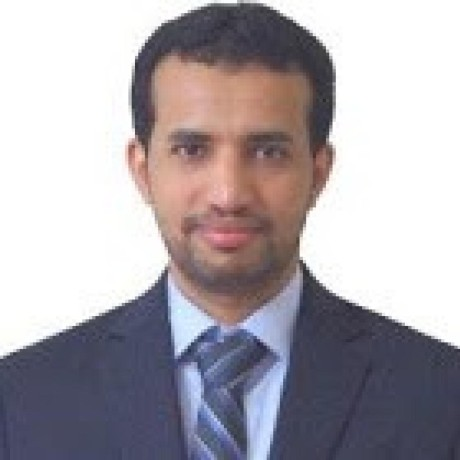
\includegraphics[width=0.30\textwidth]{images/marwan-profile.jpg}
  \caption{Marwan Alharbi, PhD student and IoT enthusiast.}
  \label{fig:marwan:profile}
\end{figure}

As a PhD student at the University of Colorado Colorado Springs (UCCS), now 
in my second year, I am committed to advancing my research in wearable 
computing. On a personal note, as a proud father of four, I balance the 
demands of family life with my academic pursuits while residing in Denver. 
In my free time, I enjoy working on IoT projects, which involve building 
printed circuit boards (PCBs) and designing 3D printed objects, including 
enclosures and moving parts. My background in web development and my 
experiments in programming languages like C/C++, Java, and Python have been 
invaluable in helping me learn algorithms and acquire skills that are 
directly applicable to my research endeavors.



\begin{figure}[h]
  \centering
  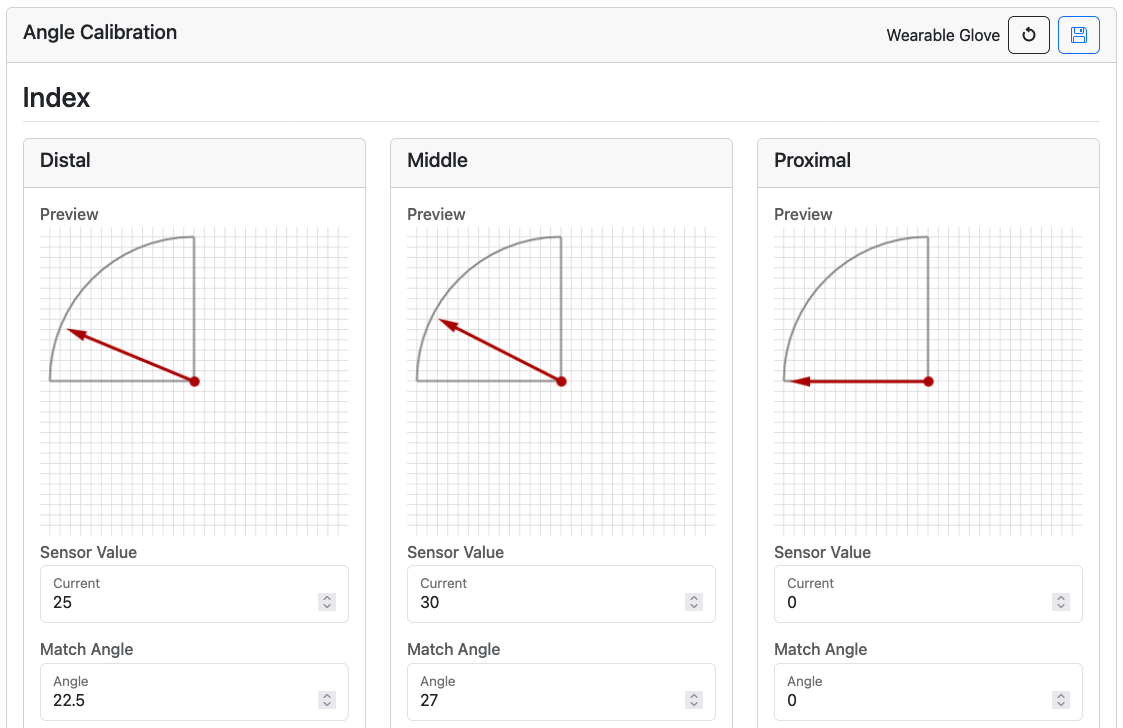
\includegraphics[width=0.90\textwidth]{images/dashboard-simulator-values.png}
  \caption{Web interface dashboard for glove sensor calibration and data management}
  \label{fig:marwan:web}
\end{figure}

\subsection{Related Implementation}
For the assignment, I chose to use my own project from the CS6770 course instead of searching for a new GitHub repository, primarily because many related GitHub projects require specialized hardware that would be difficult to acquire and test within the three-week timeframe. My project integrates several components: a glove connected to an Arduino (see Figure~\ref{fig:marwan:glove}), a controller that translates the glove's sensor data, a web interface to manage and calibrate the readings (see Figure~\ref{fig:marwan:web}), and another Arduino that controls a 3D-printed robotic finger equipped with motors to mimic the glove's movements (see Figure~\ref{fig:marwan:3d}).

\begin{figure}[h]
  \centering
  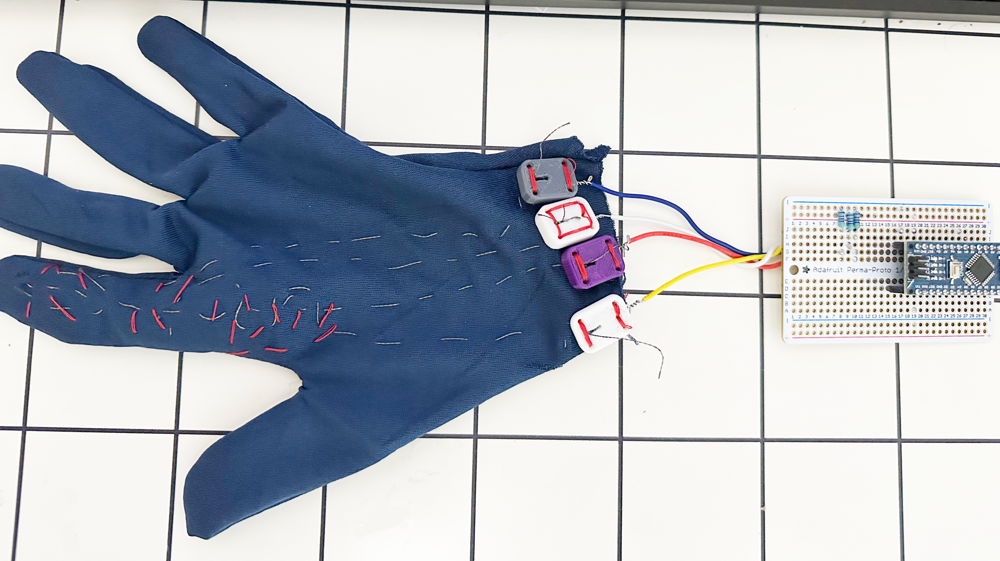
\includegraphics[width=0.80\textwidth]{images/glove-outside.png}
  \caption{Custom-made glove sensor connected to an Arduino}
  \label{fig:marwan:glove}
\end{figure}


\begin{figure}[h]
  \centering
  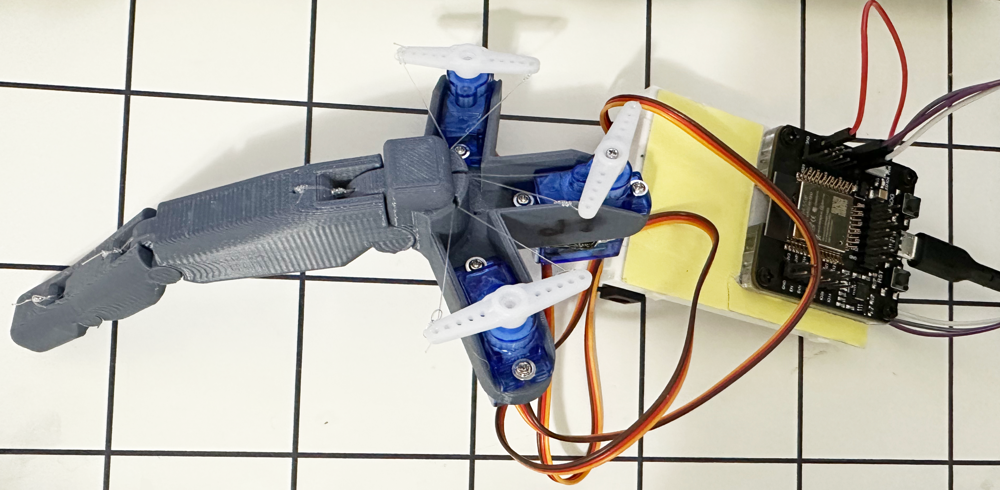
\includegraphics[width=0.80\textwidth]{images/physical-device.png}
  \caption{3D-printed robotic finger connected to motors and controlled by an Arduino}
  \label{fig:marwan:3d}
\end{figure}

In this implementation, I worked on hardware-software interaction, data transmission from the glove to the controller, and real-time visualization through the web interface. This approach allowed me to test the code using readily available equipment, focusing on translating the glove's readings into physical movements.